\chapter{Limitations in the Direct Use of the QPU}

D-Wave claims that its heuristic approach enables the search for minor embeddings computationally feasible. 
This chapter evaluates that claim to understand the limitations beyond which the QPU cannot be effectively used through a direct procedure.

As discussed in Section \ref{sec:qpuonly}, the search for an embedding is the only step that can impact the resolution speed of current quantum solvers. 
Therefore, understanding the limits of the minor embedding search corresponds to identifying the threshold beyond which the QPU cannot be used directly.

Section \ref{sec:qpu-dataset} will introduce the dataset used for testing, while Section \ref{sec:qpu-res} will present the results obtained and the corresponding analyses.

\section{Testing with Growing Problem Sizes}\label{sec:qpu-dataset}

\paragraph{Problem Size Calculation} For the formulation of the SVM problem in Equation \ref{eq:min-svm}, it is possible to calculate the number of nodes in the underlying graph of the QUBO problem. 
The only optimization variables are the $\alpha_i$ variables, one for each example. 
Since the $\alpha_i$ variables belong to the integer domain, their binary expansion must be computed for use with QUBO problems:

\begin{itemize} 
	\item Calculate the number of bits required to represent $\alpha \in [0, \text{UB}]$, i.e. $k = \lfloor\log_2(\text{UB})\rfloor + 1$; 
	\item Replace each $\alpha_i$ with $2^0\alpha_i^0 + \dots + 2^k\alpha_i^k$. 
\end{itemize}

This procedure increases the number of variables in the problem, but the new variables represent a transformation that retains all information, making them directly usable by quantum solvers.

The number of nodes in the problem is therefore:

\begin{equation}\label{eq:nodesnum}
	|\text{nodes}| = |\text{examples}|*(\lfloor\log_2(\text{UB})\rfloor + 1)
\end{equation}

Having established a measure of problem size, it is necessary to construct a dataset with controlled size increments. 
Using a synthetic dataset allows for specific and replicable tests, isolating the components currently under study.

For this reason, instead of using TweetDF, an ad hoc dataset, ToyDF, was constructed. 
This dataset does not pose a challenge for the classification procedure but is designed to be simple to create during the testing phase.

\paragraph{ToyDF Construction} To simplify the dataset as much as possible, ToyDF consists of examples positioned along the x-axis, equally divided between negative class examples, to the left of the origin, and positive class examples, to the right of the origin. 
Each example is placed at a constant distance from its neighbours or the origin, equal to one unit.

\begin{figure}[H]
    \centering
    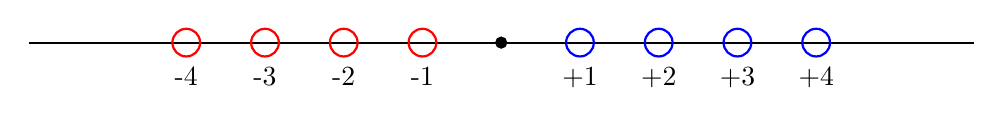
\begin{tikzpicture}
        \draw[thick] (-6,0) -- (6,0);
        \filldraw (0,0) circle (2pt);
        
        \foreach \x in {-4,-3,-2,-1} {
            \draw[red, thick] (\x,0) circle (5pt);
            \node[below] at (\x,-0.2) {\x};
	    }
        
        \foreach \x in {1,2,3,4} {
            \draw[blue, thick] (\x,0) circle (5pt);
            \node[below] at (\x,-0.2) {+\x};
 	    }
    \end{tikzpicture}
    \caption{ToyDF with 8 examples.}
    \label{fig:toydf}
\end{figure}

A structure like that in Figure \ref{fig:toydf} allows for generating a dataset that, by construction, will lead to a fixed input graph for the minor embedding algorithm. 
The number of nodes depends on only two factors:

\begin{itemize} 
	\item Equation \ref{eq:nodesnum}, where $\text{UB} = 1$ can be set to ensure that the number of nodes increases linearly with the number of examples; 
	\item The application or not of the pre-solving strategy, which, as discussed in Section \ref{sec:presolve}, doubles the number of required nodes when activated. 
\end{itemize}

SVMs generate a complete graph since each example is linked to each other. 
Although this structure is common in many optimization problems, it requires significant adjustments due to the low degree of the nodes in the Pegasus graph, as shown in Figure \ref{fig:QPU}.

\section{Results}\label{sec:qpu-res}

The search for minor embeddings was conducted with various sizes of ToyDF. 
By repeating all cases using the first 100 prime numbers as initial seeds, the results shown in Table \ref{tab:scale} were obtained.

\begin{table}[H]
    \centering
    \begin{tabular}{ccc}
        \toprule
        Problem Nodes & Average Embedding Nodes & Average Time (s) \\
        \midrule
        \rowcolor{lightgray} 4 & 4 $\pm$ 0 & 0.3 \\
        6 & 8 $\pm$ 0 & 0.2 \\ 
        \rowcolor{lightgray} 8 & 11.1 $\pm$ 1.1 & 0.5 \\ 
        % 10 & 17.5 $\pm$ 0.9 & 0.6 \\ 
        12 & 20.4 $\pm$ 0.9 & 0.5 \\ 
        \rowcolor{lightgray} 16 & 32 $\pm$ 1.1 & 0.8 \\ 
        % 20 & 47.9 $\pm$ 2.4 & 0.12 \\ 
        24 & 63 $\pm$ 2.1 & 2.4 \\ 
        \rowcolor{lightgray} 32 & 102.2 $\pm$ 5.2 & 5.6 \\ 
        % 40 & 164 $\pm$ 8.4 & 9.9 \\ 
        48 & 218.8 $\pm$ 8 & 17.1 \\ 
        \rowcolor{lightgray} 64 & 372.7 $\pm$ 27.1 & 47.1 \\ 
        % 80 & 602 $\pm$ 34.3 & 92 \\ 
        96 & 801.5 $\pm$ 56.8 & 169.1 \\ 
        \rowcolor{lightgray} 128 & 1424.5 $\pm$ 95.8 & 376.5 \\ 
        % 160 & 2205.8 $\pm$ 182.8 & 703.1 \\ 
        192 & 1696.6 $\pm$ 118.7 & 468.9 \\ 
        \rowcolor{lightgray} 256 & 3067.1 $\pm$ 213.7 & 801.3 \\
        \bottomrule
    \end{tabular}
    \caption{Minor Embedding results on ToyDF}
    \label{tab:scale}
\end{table}

The columns in Table \ref{tab:scale} indicate: 
\begin{itemize} 
	\item \textbf{Problem Nodes}: The number of nodes in the original problem; 
	\item \textbf{Average Embedding Nodes}: The number of nodes in the found embedding; 
	\item \textbf{Average Time (s)}: The time, in seconds, taken to find the embedding. 
\end{itemize}

The highlighted rows represent problems where the initial problem size is a power of two. 
Although this characteristic does not have significant consequences for the analysis, doubling the required number of nodes is not uncommon. This doubling can be due to:
\begin{itemize} 
	\item Use of pre-solving; 
	\item An increase in the upper bound of the $\alpha_i$ variables, which in an ideal (error-free) SVM scenario should be able to tend toward $+\infty$. 
\end{itemize}

Figure \ref{fig:scale_nodes} shows the number of QPU nodes required to find an embedding for the graph. 
Given the difference in scale between the x-axis and y-axis, it can be observed that the demand for nodes grows exponentially.

For instance, a problem with 256 nodes, an insignificant dataset size compared to TweetDF, requires 3,000 qubits on the QPU. 
Given that current D-Wave QPUs have around 5,600 qubits, it is unlikely that an embedding will be found for larger problems.

\begin{figure}[H] 
	\centering 
	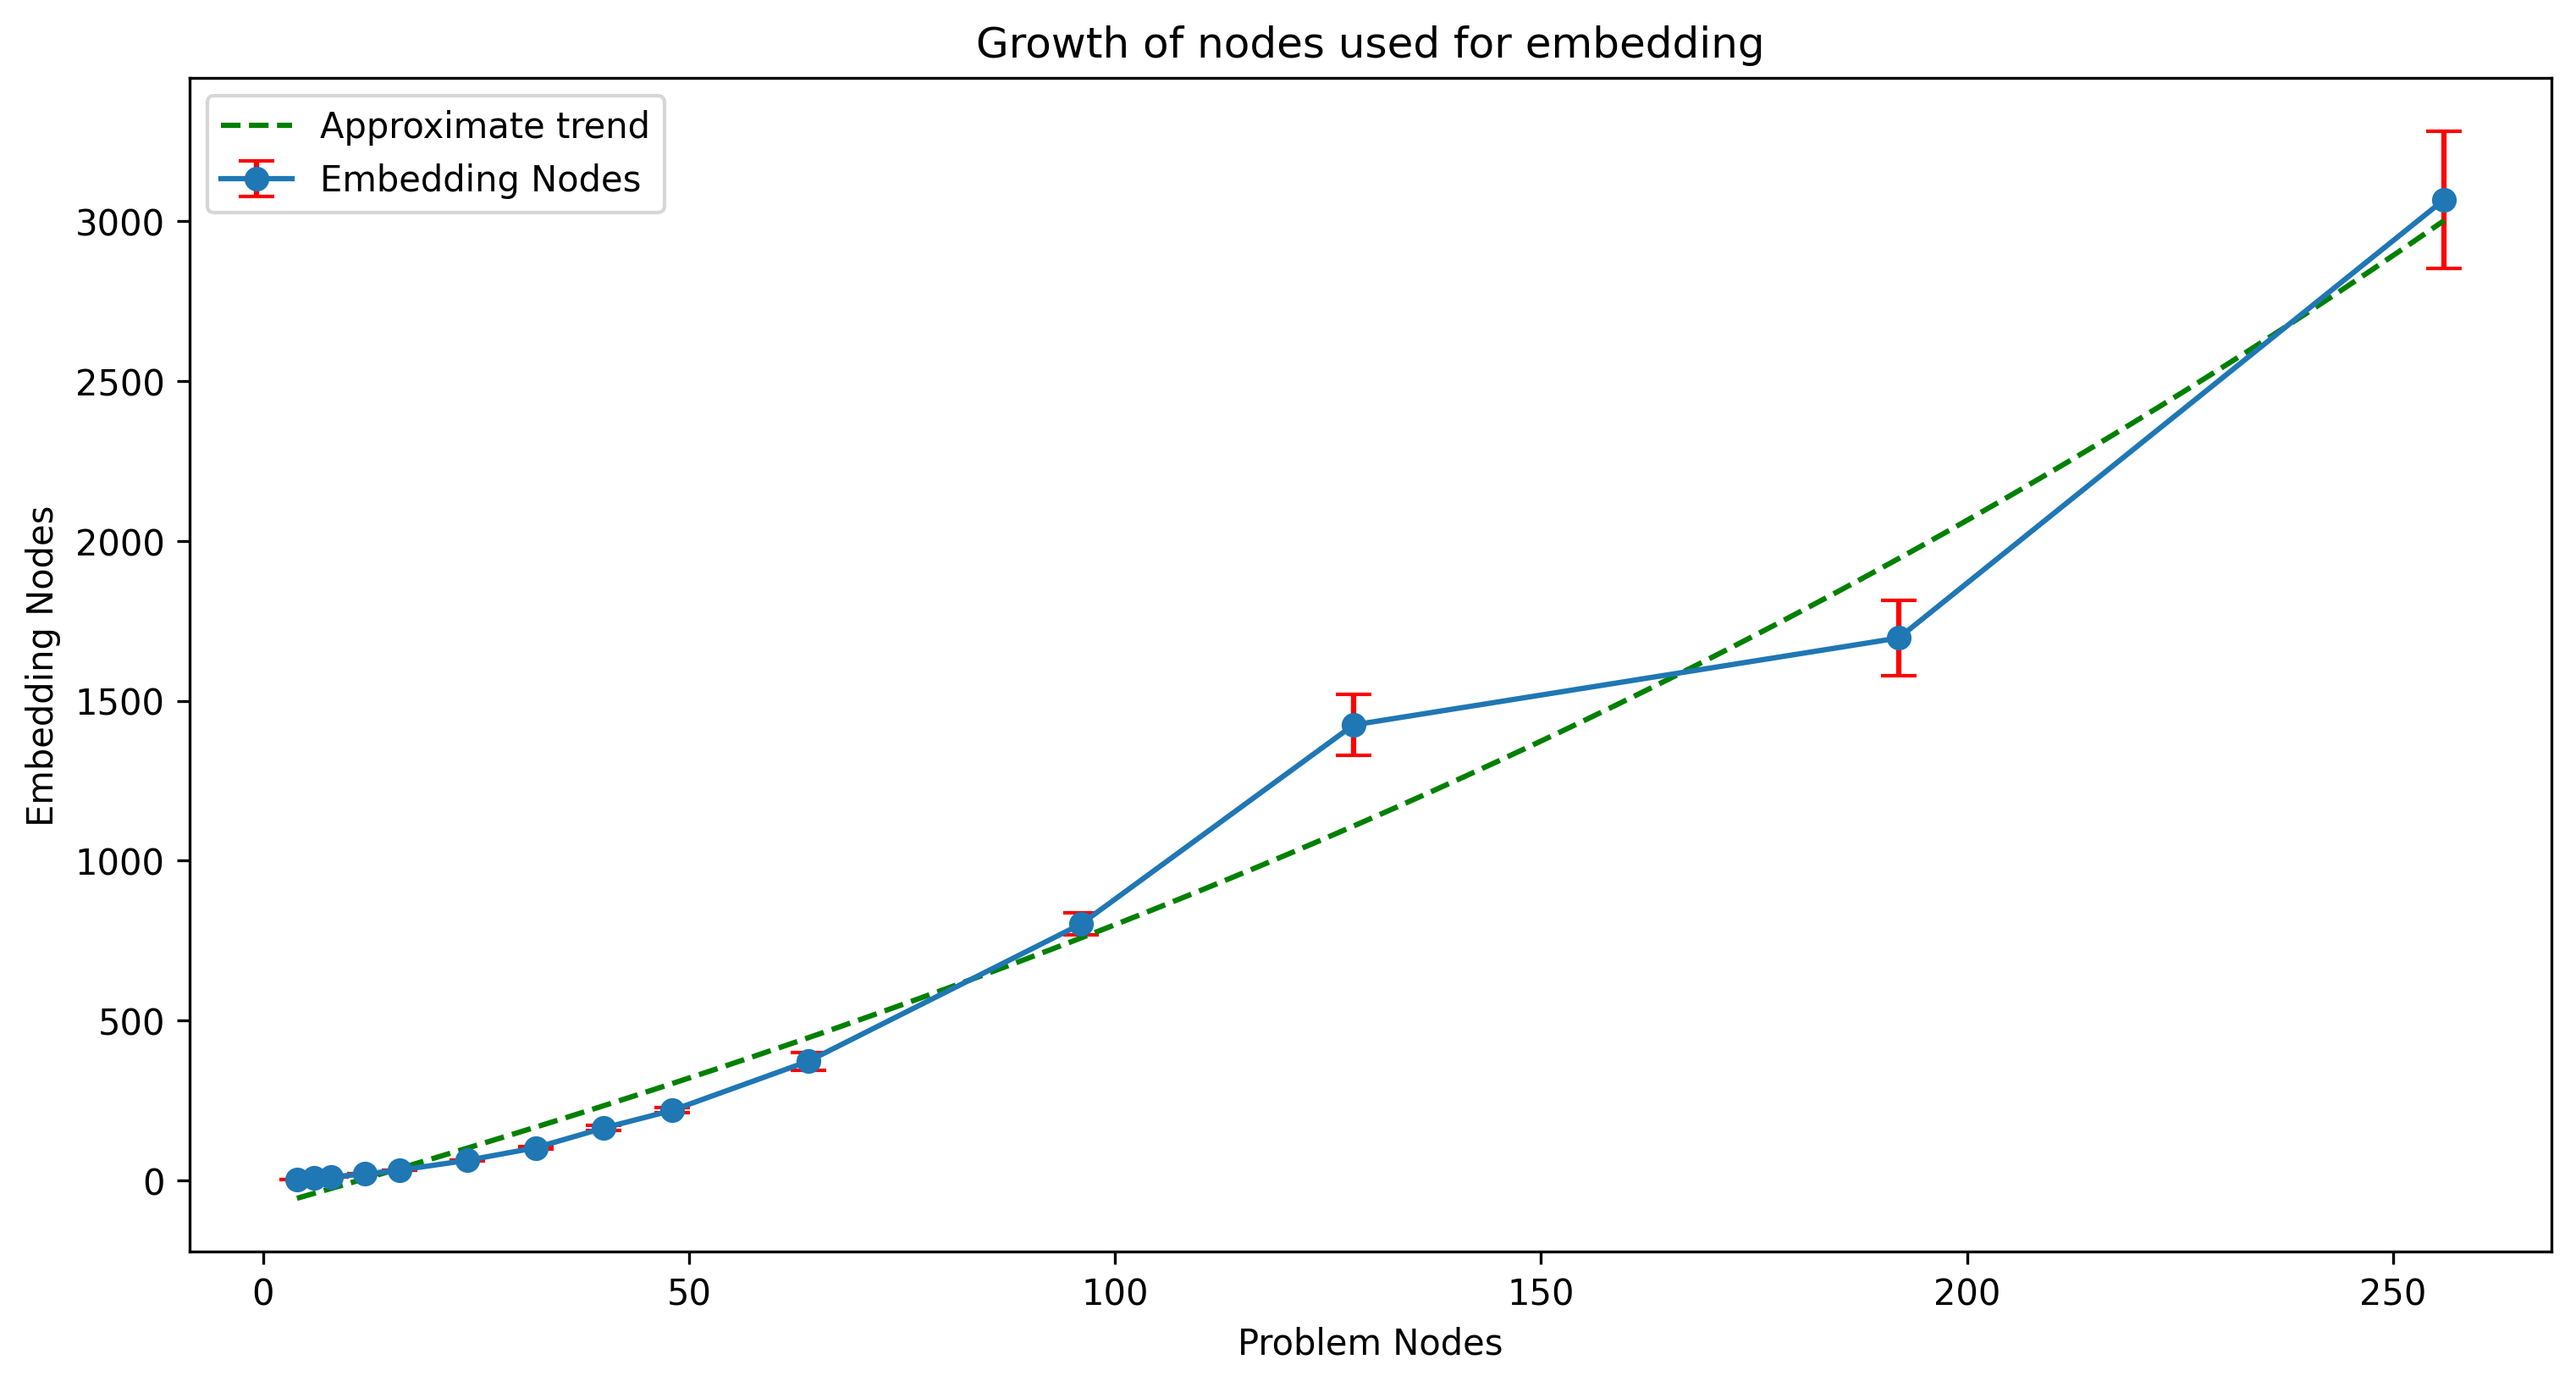
\includegraphics[width=\textwidth]{figures/scale_node.png} 
	\caption{Growth of nodes used for embedding.}
	\label{fig:scale_nodes}
\end{figure}

Figure \ref{fig:scale_time} shows the average time required to compute the embedding. 
Although the growth is not exponential, the complexity of the procedure significantly impacts performance, reaching 800 seconds for moderately sized problems.

Given that these times refer to a preprocessing operation, such high values are incompatible with the results recorded in Section \ref{sec:qsvm-performance}. 
In the case of the hybrid solver, the time recorded to compute the optimal solution with 4,096 examples and an upper bound of $\alpha = 255$ is less than the time required for the minor embedding search for problems with 128 nodes.

\begin{figure}[H] 
	\centering 
	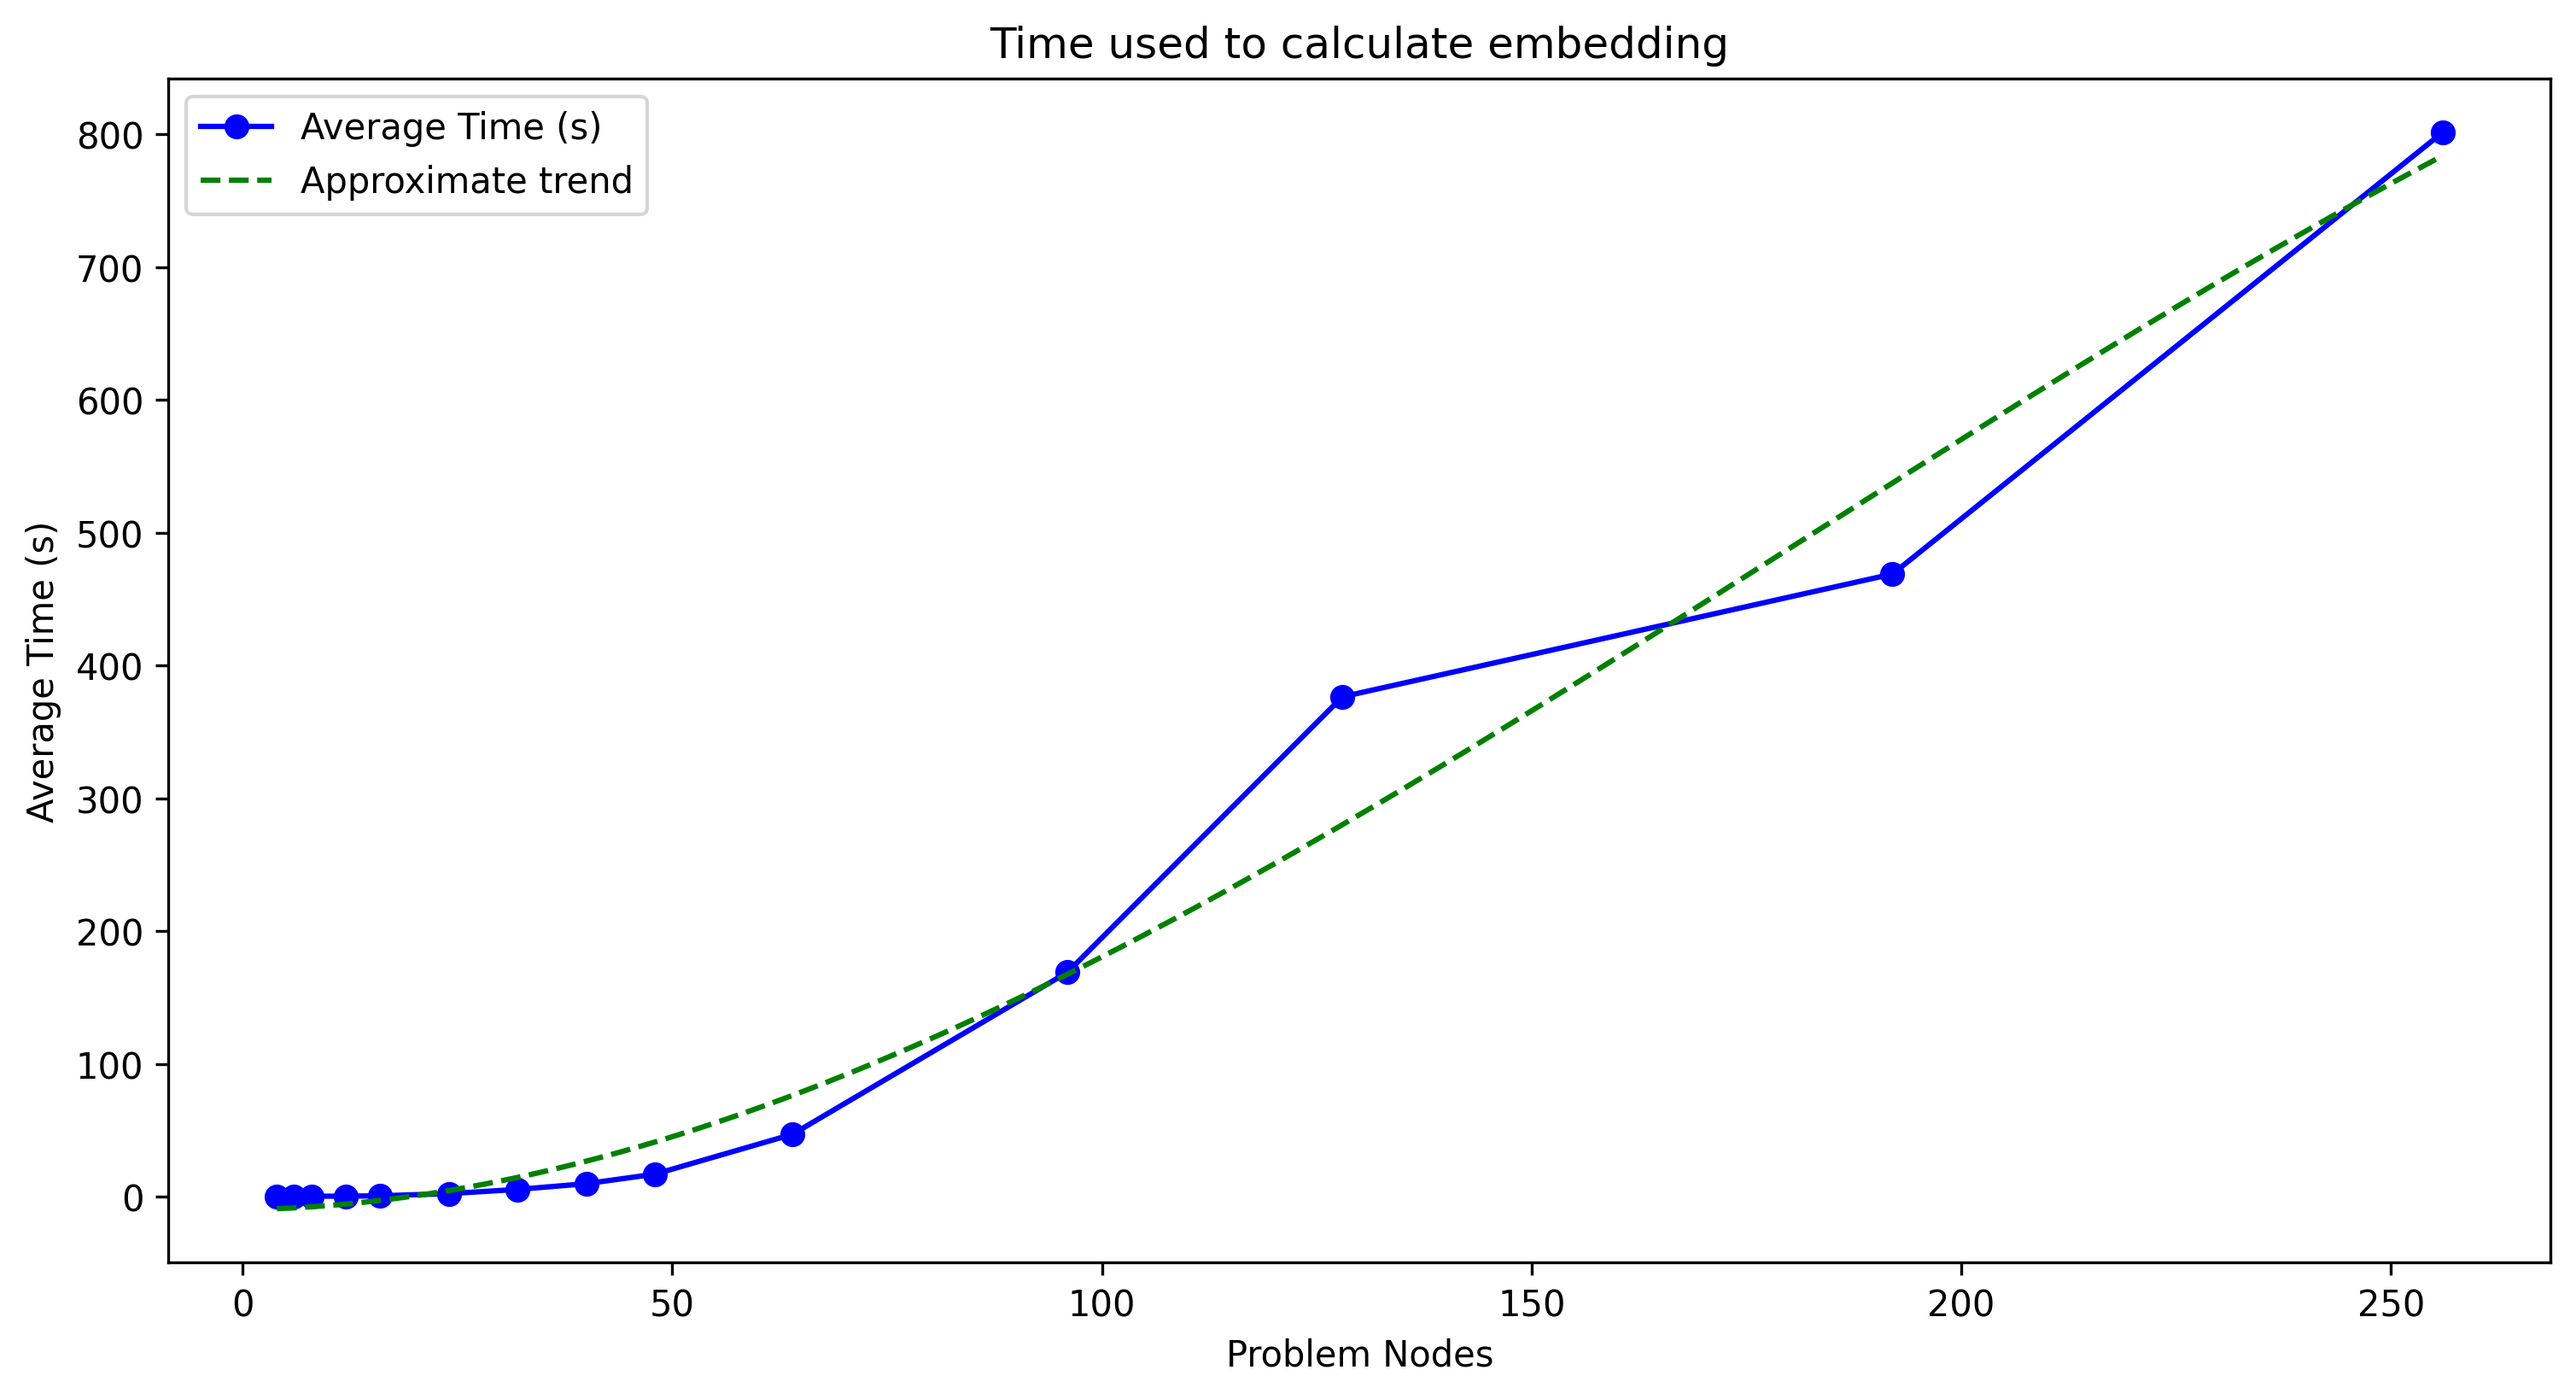
\includegraphics[width=\textwidth]{figures/scale_time.png} 	
	\caption{Time required to calculate embedding.} 
	\label{fig:scale_time}
\end{figure}

\subsection{QPU Solver vs. Hybrid Solver}

These findings indicate that the direct use of the QPU is not a scalable alternative capable of solving problems beyond those currently addressed by classical computers.

The use of hybrid solvers is therefore a key step for the optimal utilisation of quantum annealing technology. 
It is therefore worth considering whether alternative hybrid solvers can be developed to further exploit the QPU and improve performance in problem-solving.